\subsection{1.3 Large Beam Bending}
\label{sec:large_beam_bending}
\framecard{1.3 Large Beam Bending}
\begin{frame}{Set up}
	\bfc{\igwf{configuration_large_beam_bending.eps}{110mm}}{Set up [Credits: G. Puel]}{}
\end{frame}

% Set up
\begin{frame}{Set up}
\txb{120}{3}{12}{
	\begin{block}{Kinematic description}
		\begin{itemize}
			\item $\pv=p_1\ione+p_2\itwo$; $(p_1,p_2)\in \left]-h,h\right[ \times \left]0,L\right[$
			\item $\xv[]\pptp=\xv[G]\pdp{p_2,t}+p_1\ir\pdp{\theta\pdp{p_2,t}}$
		\end{itemize}
	\begin{center}
		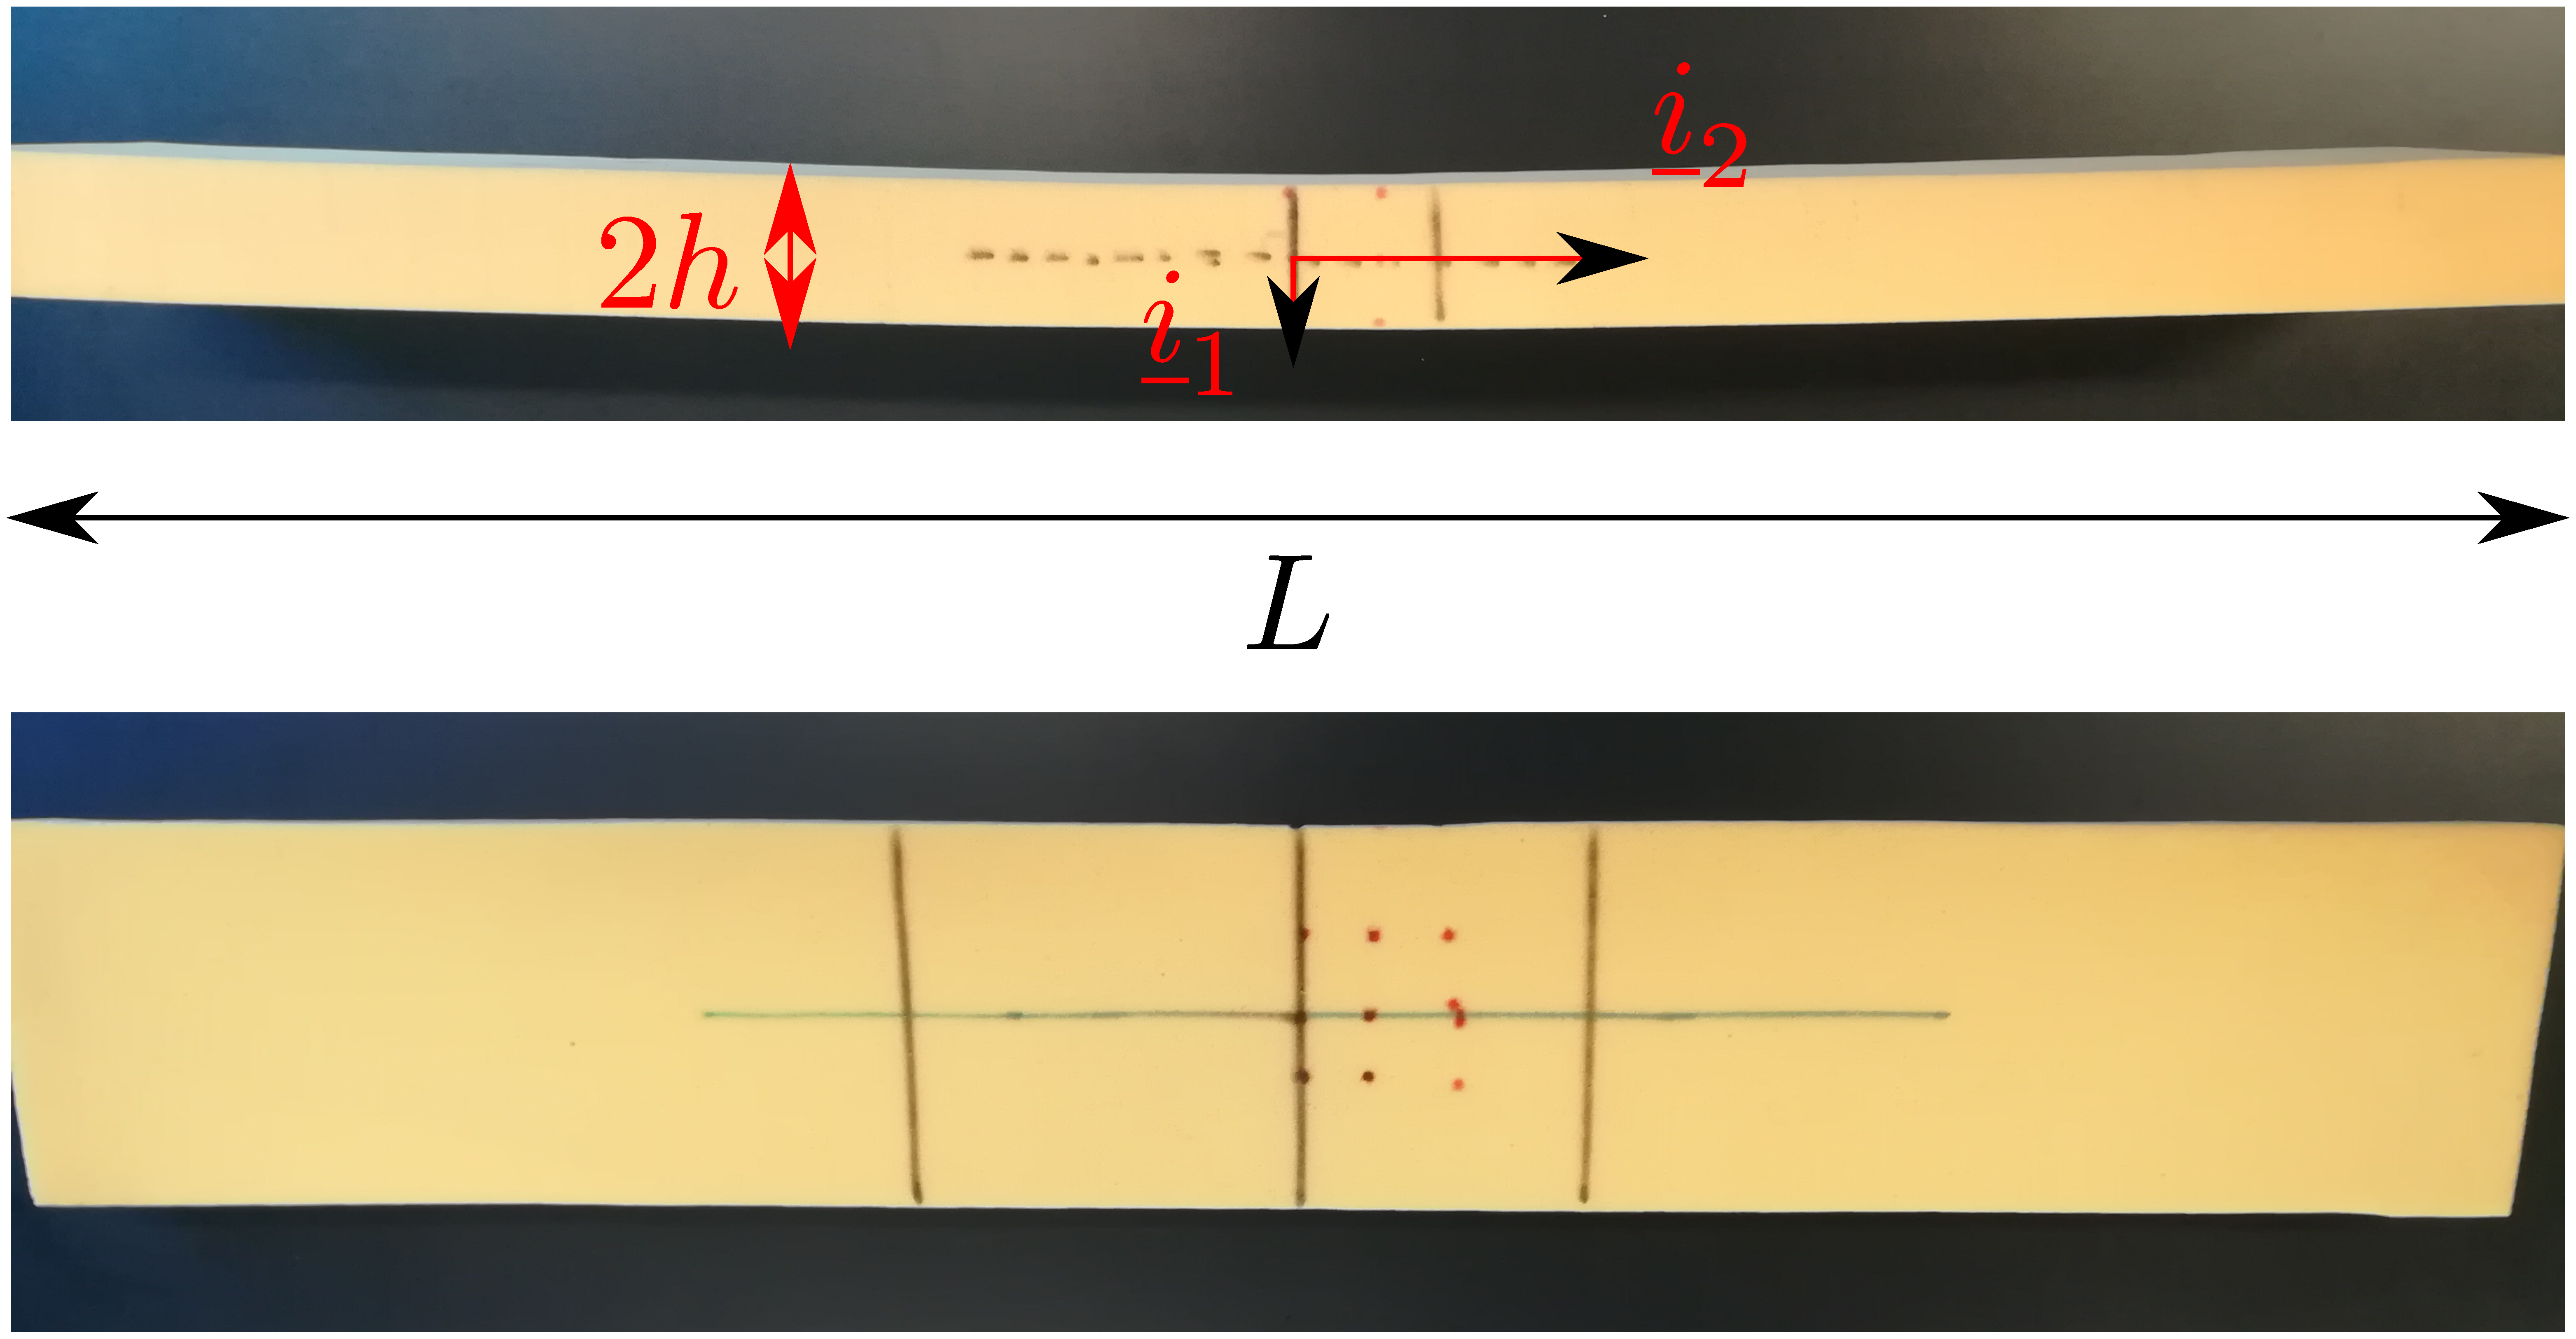
\includegraphics[width=65mm]{large_beam_bending_1.eps}
	\end{center}

		\end{block}
}
\end{frame}


\begin{frame}{Set up}
	\txb{120}{3}{12}{
		\begin{exampleblock}{Question 1: physical interpretation}
			\begin{itemize}
				\item $p_1=0\Rightarrow \xv=\xv[G]$ (middle line deflection)
				\item  $p_1\ir\pdp{\theta\pdp{p_2,t}}$ : cross-section rotation
			\end{itemize}
			\begin{center}
				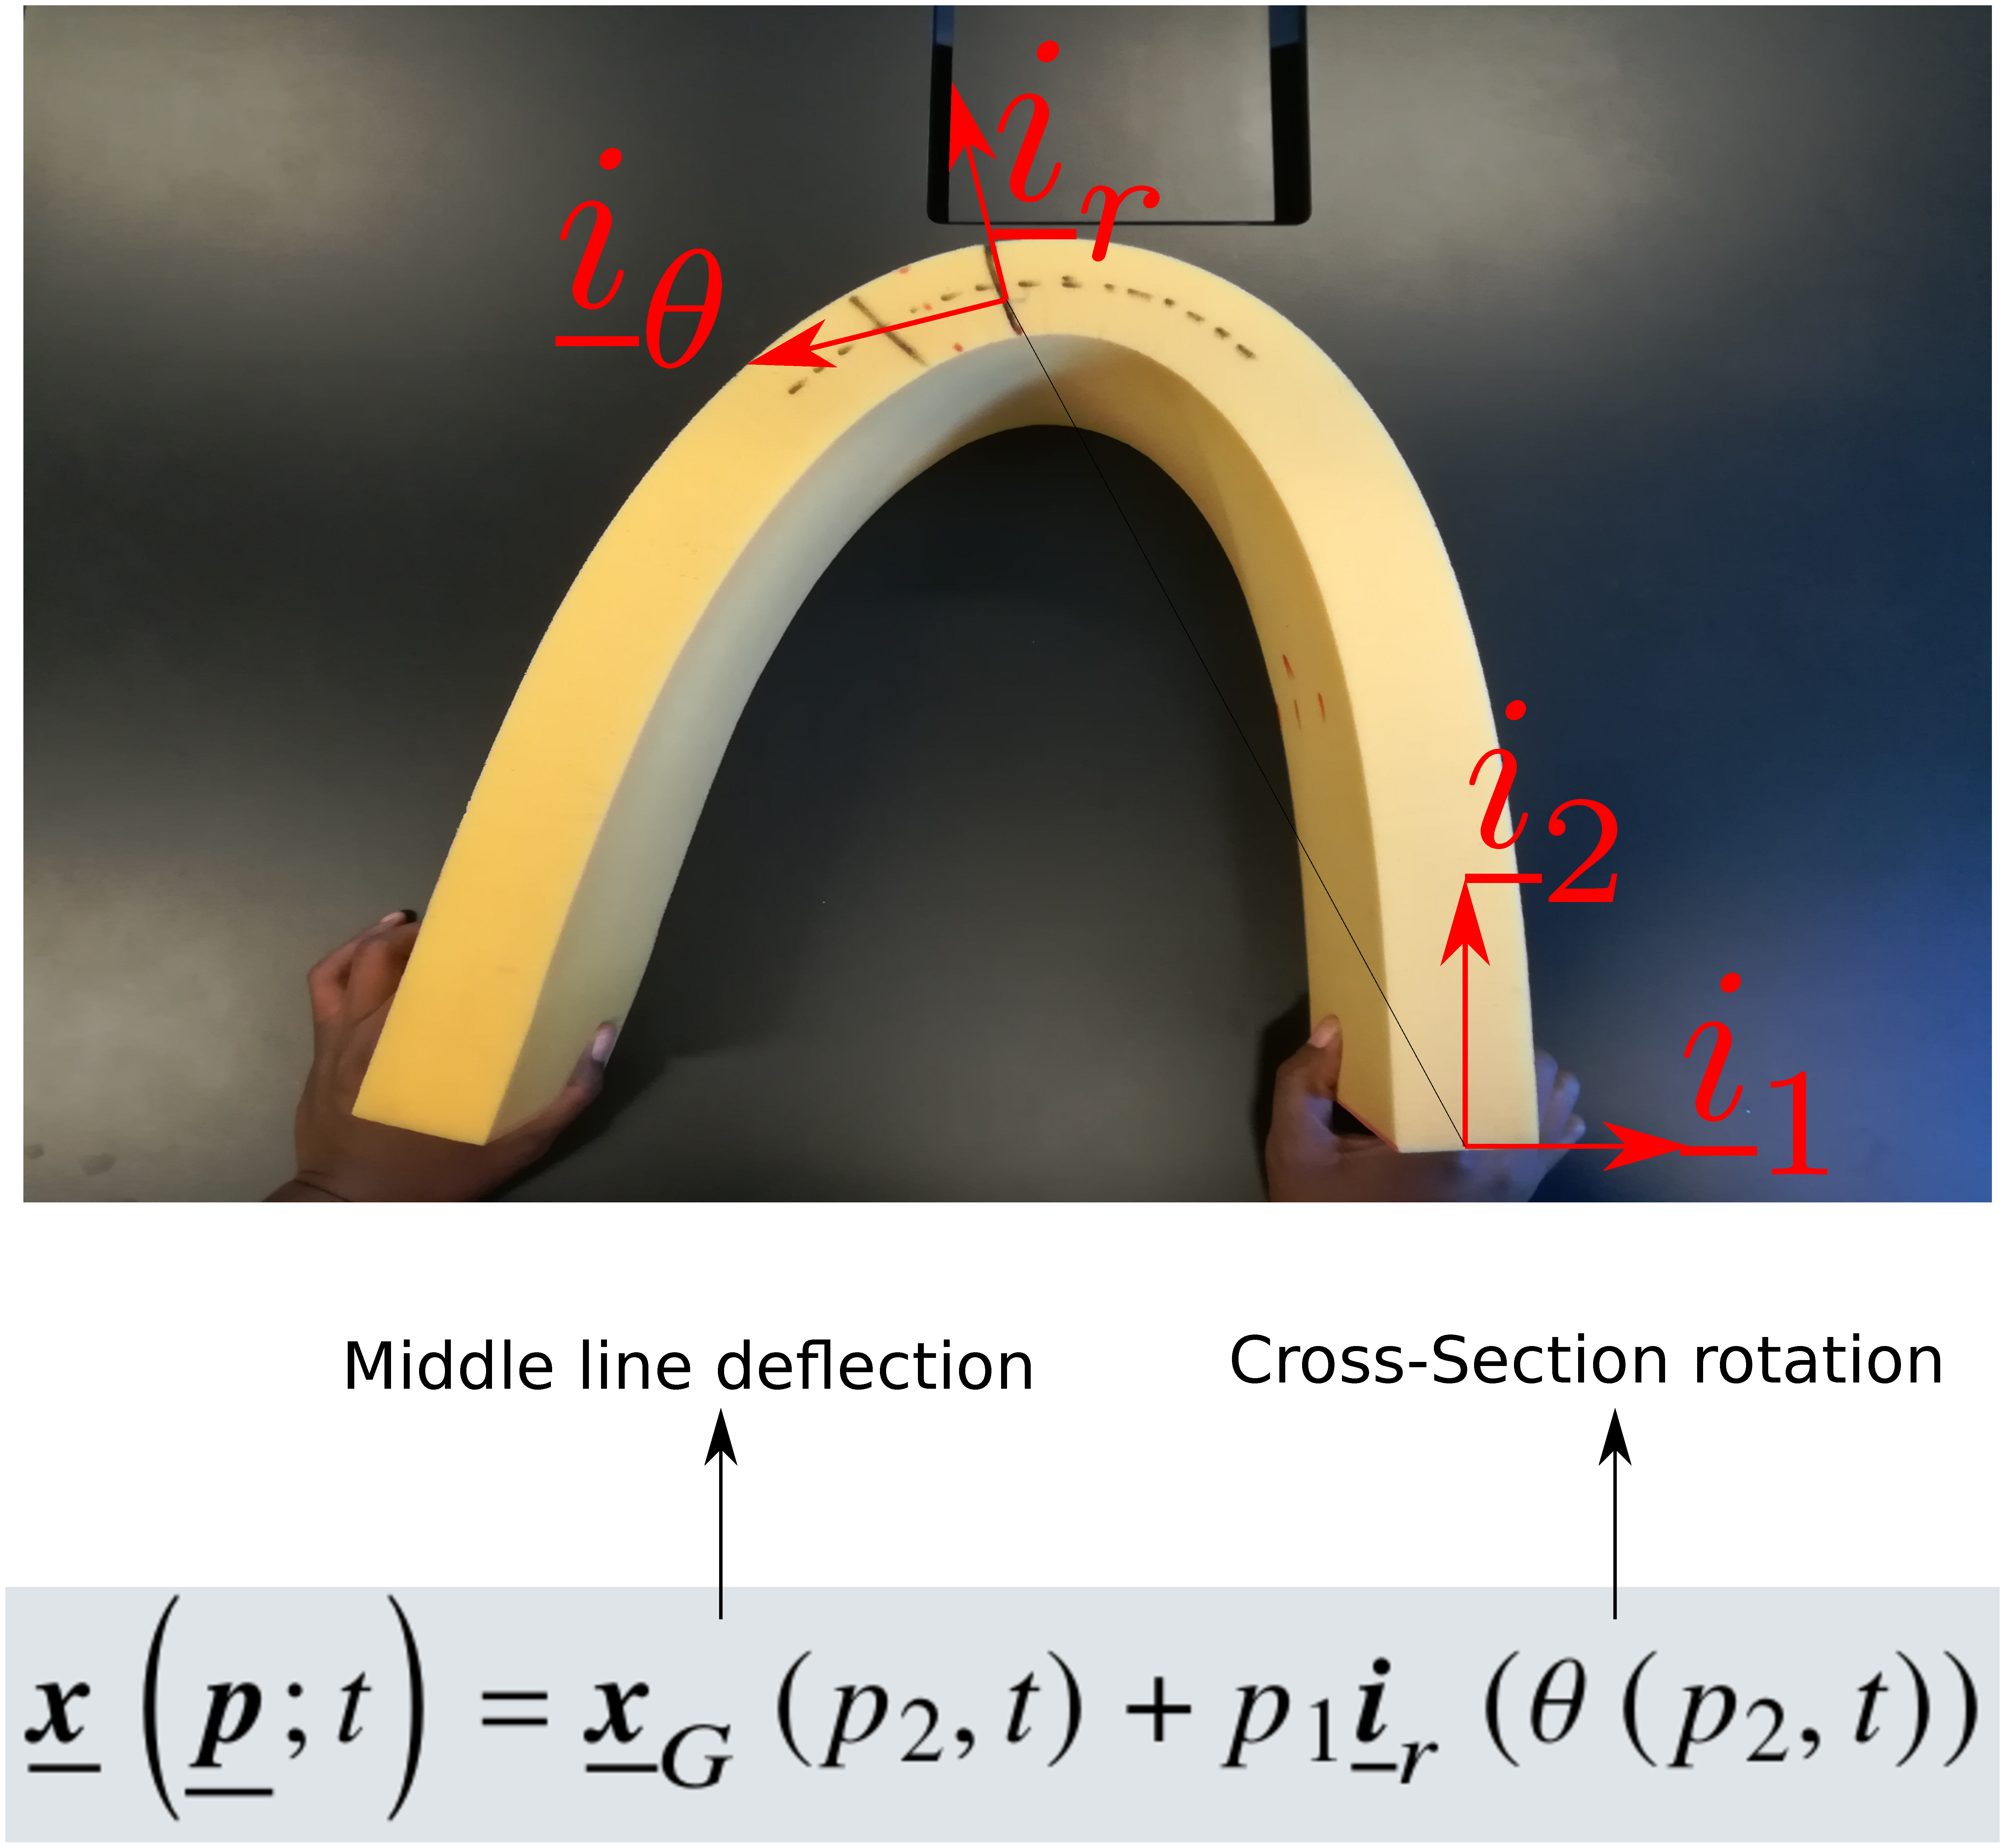
\includegraphics[width=60mm]{large_beam_bending_2.eps}
			\end{center}
			
		\end{exampleblock}
	}
\end{frame}

% Recap F and FT
\begin{frame}{Displacement and Space Gradient}
	\only<1>{
		\bfc{\igwf{configuration_gradient}{110mm}}{Tenseur gradient [Credits: G. Puel]}{}
	}
	\only<2>{
		\begin{itemize}
			\item Displacement vector:
			\beq{\uv\pptp=\xv\pptp-\pv=\vct{f}{}{}\pptp-\pv}{}
			\item Space gradient tensor: \beq{\vct{dx}{}{}=\Fgrad.\vct{dp}{}{},\quad \vct{du}{}{}=\pdp{\Fgrad-\ID}\vct{dp}{}{}}{dxFdp} 
		\end{itemize}
		\textit{The displacement gradient tensor maps tangent vector from $\kappa_0$ into $\kappa_t$.}	
		\beq{\Fgrad=\cartFgrad}{Fexp}
		\beq{\Fgrad=\curvFgrad}{Fcurv}\\ \hspace{-2mm}\vspace{5mm} curvilinear coordinates $\xi_i$
	}
\end{frame}


% Compute F and FT
\begin{frame}{Transformation Gradient}
	\txb{120}{3}{12}{
		\begin{block}{Compute space gradient}
			\only<1->{
			$$\pard[\xv][p_1]=\ir\pdp{\theta\pdp{p_2,t}}\quad\quad \pard[\xv][p_2]=\pard[\xv[G]][p_2]\pdp{p_2,t}+p_1\pard[\theta][p_2]\pdp{p_2,t}\ith\pdp{\theta\pdp{p_2,t}}$$
		}
			\only<2->{
			\beq{
				\begin{split}
					\Fgrad = \otp[\pard[\xv][p_1]][\ione]+\otp[\pard[\xv][p_2]][\itwo]=& \\  =\ir\pdp{\theta\pdp{p_2,t}}\otimes\ione+\pard[\xv[G]][p_2](p_2)\otimes \itwo +& p_1\pard[\theta][p_2]\pdp{p_2,t} \ith\pdp{\theta\pdp{p_2,t}}\otimes \itwo
				\end{split}
			}{Fgrad}
		}
	\only<3->{
		\begin{scriptsize}
			\beq{
				\FgradT = \otp[\ione][\ir\pdp{\theta\pdp{p_2,t}}]+ \itwo\otimes\pard[\xv[G]][p_2](p_2) + \itwo\otimes p_1\pard[\theta][p_2]\pdp{p_2,t} \ith\pdp{\theta\pdp{p_2,t}}
			}{FgradT}
		\end{scriptsize}
	}
		\end{block}
	}
\end{frame}

% Recap Green-Lagrange tensor
\begin{frame}{Large Strains}
		\bfc{\igwf{configuration_green_lagrange}{40mm}\\
			\ighf{dx1dx2_dp1dp2}{30mm}\vspace{-3mm}}{\textit{Measure} of the deformation [Credits: G. Puel]:\\ Stretch [top] - Angular distortion [down]}{}
\end{frame}


%Measure large strain via Green-Lagrange tensor
\begin{frame}{Measure the large strains}
		\txb{123}{0}{9}{
			\hspace{-2mm}
			\begin{itemize}
				\itemsep0em 
				\item Green-Lagrange tensor:\vspace{-3mm} \beq{\Estrain=\FEstrain=\UEstrain}{Estrain}\vspace{-3mm}
				\item Stretching of a fiber $dp\vct{e}{p}{}$:
				\beq{\frac{\norm{\vct{dx}{}{}}^2-\norm{\vct{dp}{}{}}^2}{\norm{\vct{dp}{}{}}^2}=2\pscl{\vct{e}{p}{}}{\Estrain \vct{e}{p}{}} = 2 \mathbb{E}_{pp} }{dx2dp2} \vspace{-3mm}
				\item Angular distortion of two fibers $dp_1\vct{e}{p1}{}$ $dp_2\vct{e}{p2}{}$:
				\beq{ \hspace{-3mm}\sin\pdp{\gamma_{12x}} = \cos\pdp{\alpha_{12x}} = {\scriptscriptstyle  \frac{\pscl{\pdp{2\Estrain+\ID}\vct{e}{p1}{}}{\vct{e}{p2}{}}}{\sqrt{
								\pscl{\pdp{2\Estrain+\ID}\vct{e}{p1}{}}{\vct{e}{p1}{}}
							}\sqrt{
								\pscl{\pdp{2\Estrain+\ID}\vct{e}{p2}{}}{\vct{e}{p2}{}}	
					}}  } = \frac{2\mathbb{E}_{12}+1}{\sqrt{\pdp{2\mathbb{E}_{11}+1}\pdp{2\mathbb{E}_{22}+1}}} }{sinEstrain}
			\end{itemize}
		}
	\txb{30}{2}{75}{
		\ighf{angular-distorsion}{15mm}
	}
	
\end{frame}

% Compute Green-Lagrange tensor
\begin{frame}{Green-Lagrange tensor}
	\txb{120}{3}{12}{
		\begin{exampleblock}{Question 2: Compute Green-Lagrange tensor}
			\beq{
				\begin{split}
					\Cstr =\FgradT.\Fgrad \quad&\quad \Estrain = \frac{1}{2}\pdp{\Cstr-\ID}\\
					\Estrain = \pscl{\pard[\xv[G]][p_2]}{\ir}\ione\sotp\itwo +& \frac{1}{2}\pdp{\pdp{\pard[\xv[G]][p_2]+p_1\pard[\theta][p_2] \ith}^2-1 }\otp[\itwo][\itwo]
				\end{split}
			}{Cstr}
		\end{exampleblock}
	}
\end{frame}


% Example Green Lagrange tensor
\begin{frame}{What does $\Estrain$ measure?}
		\bfc{\ighf{example-green-lagrange}{65mm}}{Credits: G. Puel.}{example-green-lagrange}
\end{frame}


% Large beam bending : Stretching and Distortion
\begin{frame}{Physical interpretation}
	\txb{120}{3}{12}{
		\begin{exampleblock}{Question 3: Compute $E_{11}$}
			\begin{itemize}
				\item $E_{11}= 0, \lambda_{11}=\sqrt{C_{11}}=1$ no stretching along $\ione$
				\item $E_{22}=\frac{1}{2}\pdp{\pdp{\pard[\xv[G]][p_2]+p_1\pard[\theta][p_2] \ith}^2-1 }$, $\lambda_{22}=\sqrt{C_{22}} = \Big\Vert\pard[\xv[G]][p_2]+p_1\pard[\theta][p_2] \ith\Big\Vert$
				\item $E_{12}= \frac{1}{2}\pscl{\pard[\xv[G]][p_2]}{\ir}$, $\cos\pdp{\alpha_{x12}}=\frac{2\pscl{\pard[\xv[G]][p_2]}{\ir}+1}{\Big\Vert\pard[\xv[G]][p_2]+p_1\pard[\theta][p_2] \ith\Big\Vert}$
			\end{itemize}
		\end{exampleblock}
	}
\end{frame}


% Large beam bending : Stretching and Distortion
\begin{frame}{Half-circle deflection}
	\txb{120}{3}{12}{
		\begin{block}{Half-circle middle line deflection}
			\begin{itemize}
			\item $\xv[G]\pdp{p_2}=\frac{L}{\pi}\pdp{-\ione+\ir\pdp{\theta\pdp{p_2}}}$
				\item $\theta\pdp{p_2}=\frac{\pi}{L}p_2$
			\end{itemize}
		\end{block}
	\begin{exampleblock}{Question 4: Physical interpretation}
				\ighf{large_beam_bending_3.eps}{45mm}
		\end{exampleblock}
	}
\txb{50}{75}{45}{
	\begin{itemize}
		\item $\theta(0)=0,\quad \theta(L) = \pi$
		\item $\xv[G]$ describes a circle!
		\item $\pard[\xv[G]][p_2]=\ith$
	\end{itemize}
}
\end{frame}


% Physical interpretation for half-circle
\begin{frame}{Physical interpretation}
	\txb{120}{3}{12}{
		\begin{exampleblock}{Questions 5/6: Compute $E_{22}, E_{12}$}
			\begin{itemize}
				\item $E_{11}= 0, \lambda_{11}=\sqrt{C_{11}}=1$ no stretching along $\ione$
				\item $E_{22}=\frac{1}{2}\pdp{\pdp{1+p_1\frac{\pi}{L} }^2-1 }$, $\lambda_{22}=\sqrt{C_{22}} = \Big\vert1+p_1\frac{\pi}{L} \Big\vert$
				\item $E_{12}= \frac{1}{2}\pscl{\pard[\xv[G]][p_2]}{\ir}=0$, $\cos\pdp{\alpha_{x12}}=\frac{1}{\Big\vert1+p_1\frac{\pi}{L} \Big\vert}$\\ No deflection: Cross-section $\perp$ to middle-line!
			\end{itemize}
		\end{exampleblock}
	}
\end{frame}

% Physical interpretation for half-circle with deflection
\begin{frame}{Physical interpretation}
	\txb{120}{3}{12}{
		\begin{exampleblock}{Question 7: Compute $E_{11}, E_{22}, E_{12}$}
			\centering
			\igwf{large_beam_bending_4.eps}{100mm}
		\end{exampleblock}
	}
\end{frame}

% Small strain theory
\begin{frame}{Small Displacements/Strains}
	\txb{110}{0}{11}{
		\begin{itemize}
			\item Small Displacements/Small Strains:	\beq{\max_{\pxtp}\norm{\uv} << \mathcal{L} \pdp{\xv\approx\pv}, \quad \max_{\pxtp}\norm{\gradt{u}{p}}^2=Tr\pdp{\gradpUT\gradpU}<<1}{petitDepDef} 
			\item Small Strain tensor:
			\beq{\Estrain\approx\strain=\frac{1}{2}\pdp{\gradt{u}{x}+\gradtT{u}{x}} =\cartEspilon}{smallStrain}
			$$\frac{\Delta l}{l_0} = \pscl{\vct{e}{}{}}{\depsil \vct{e}{}{}}=\depsil_{ee},\quad \frac{\Delta\gamma_{12}}{2}=\pscl{\vct{e}{1}{}}{\depsil \vct{e}{2}{}}=\depsil_{12}$$
			\item Local volume change:
			\beq{\evol=\frac{\Delta V}{V_0}=\frac{l_{01}+\Delta l_1}{l_{01}}\frac{l_{02}+\Delta l_2}{l_{02}}\frac{l_{03}+\Delta l_{03}}{l_{03}} \approx Tr\pdp{\depsil}}{epsvol}
		\end{itemize}
	}
	\txb{15}{110}{11}{
		\igwf{small-displ}{15mm}
	}
\end{frame}

% Small strain beam 
\begin{frame}{Small-strain tensor}
	\txb{120}{3}{12}{
		\begin{exampleblock}{Question 8: Compute $\strain$}
			\begin{itemize}
				\item $\uv\pdp{\pv,t}=\uv[G](p_2,t)+p_1(\ir-\ione)$
				\item $\norm{\uv}\ll h\Rightarrow\uv\approx\uv[G]\ll h$
				\item $p_1\in\left]-h,h\right[$, with $h<L$ and $\theta\ll 1,\quad \ir\approx \ione$
				\item $\norm{\gradpU}\ll 1\Rightarrow \norm{\pard[\uv[G]][p_2]}\ll 1,\quad \pard[\theta][p_2]\ll 1$
				
				\item $\depsil_{11}=0$: no elongation along $\ione$
				\item $\depsil_{22}=\pard[u_{G,2}][p_2]+p_1\pard[\theta][p_2]$ : linear elongation (with $p_1$) along $\itwo$
				\item $\depsil_{12}=\frac{\pard[u_{G,1}][p_2]+\theta}{2}$: no distortion if $\pard[u_{G,1}][p_2]=\theta$ (Euler Bernoulli assumption)
			\end{itemize}
		\end{exampleblock}
	}
\end{frame}




